\documentclass[mla8]{mla}
\usepackage[T1]{fontenc}

% Command to print word count
\newcommand\wordcount{\input{wqu-words.sum}}
\newcommand\wordcounts{\input{wqu-heads.sum}}
\newcommand\wordcountt{\input{wqu-text.sum}}

% Modify the title
\title{
\includegraphics[width=2.5cm]{WQU_Radial-Icon_FullColor_RGB.png}\\[0.5cm]\MakeUppercase{MScFE 560 Financial Markets :\newline Title}}

% Modify authors
\author{Author: Anonymous}

% Set compile time date
\date{\mladate} % see docs for `\mladate'

\addbibresource{wqu.bib} %Imports bibliography file

\begin{document} 
% No need to use maketitle since the MLA class takes care of it

% The following comment avoids to count word in notes
%TC:macro \endnote [ignore]

%TC:ignore
% Count words and save result in file
\immediate\write18{texcount -nc -nobib -sum=1,1 -1 wqu.tex  > wqu-words.sum}
\immediate\write18{texcount -nc -nobib -sum=0,1 -1  wqu.tex  > wqu-heads.sum}
\immediate\write18{texcount -nc -nobib -sum=1 -1  wqu.tex  > wqu-text.sum}
%TC:endignore

\begin{paper}

%TC:ignore

\begin{abstract}

This is the abstract. Each section between commands \textbf{\%TC:ignore} and \textbf{\%TC:endignore} is excluded from the word count.
\end{abstract}

\bigskip

\noindent{Total words excluding heading, title, author, abstract, introduction, conclusion, notes, captions and references (but including section titles): \textbf{\wordcount} of which \wordcounts as section titles and \wordcountt as text (required words: 1,000 ± 200).}

\noindent{\rule[0.5ex]{\linewidth}{1pt}}

%TC:endignore
%TC:ignore
\setlength{\parindent}{2em}
\section*{Introduction}
\indent
The introduction is not counted in the word count\endnote{This is a note} and this is a citation with page number, optional \parencite[p.~200]{mishkin_eakins_2018}. 

We can reference a figure (Fig.~\ref{fig:overleaf}) and the number will be updated automatically. The \textbf{\textasciitilde} inserts a non breakable space.
% Example figure
\begin{figure}[H]
	\centering
	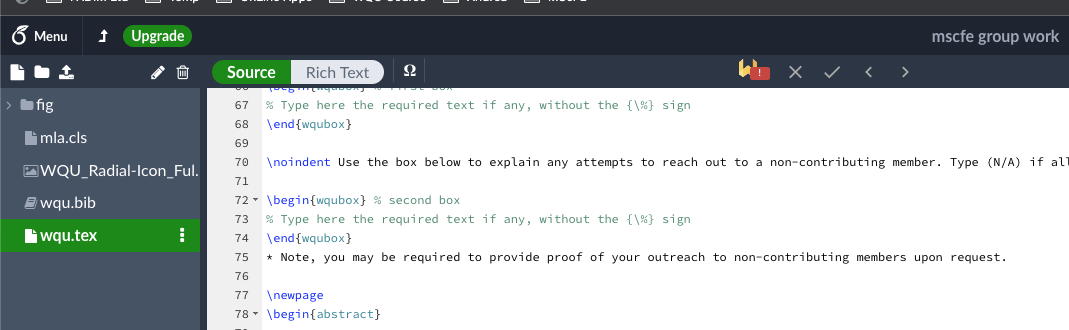
\includegraphics[width=\columnwidth]{fig/overleaf.png}
	\caption{Create a project with the name you like and copy in it the files including the fig folder.\\ Data Source: Overleaf \href{https://www.overleaf.com?r=049a7499&rm=d&rs=b}{https://www.overleaf.com}}
	\label{fig:overleaf}
\end{figure}


%TC:endignore


\section*{Section title}
The words in this section are counted. You can also add \textit{subsections}.
\subsection{ This is a subsection}
\subsubsection{This is a sub subsection}
If you want also \textit{subsubsection} are available as well as list
\begin{itemize}
    \item one
    \item two
    % sublists
    \begin{itemize}
        \item three
        \item four
    \end{itemize}
\end{itemize}



\section*{Section title two}
If you remove the asterisk after the command section they will be automatically numbered. Another citation without page number \parencite{mishkin_eakins_2018}. Pleas note that endnotes, references and citations are actually hyperlinks. Click on them and you will go to the correct position.

A numbered list:
\begin{enumerate}
    \item one
    \item two
    \begin{enumerate}
        \item three
        \item four
    \end{enumerate}
\end{enumerate}

%TC:ignore
\section*{Conclusion}
Also the conclusion is not counted in the word count. 
%TC:endignore

\end{paper}

\begin{notes}
\printendnotes
\end{notes}

\begin{workscited}
\printbibliography[heading=none]
\end{workscited}

\end{document}